% Options for packages loaded elsewhere
% Options for packages loaded elsewhere
\PassOptionsToPackage{unicode}{hyperref}
\PassOptionsToPackage{hyphens}{url}
\PassOptionsToPackage{dvipsnames,svgnames,x11names}{xcolor}
%
\documentclass[
  letterpaper,
  DIV=11,
  numbers=noendperiod]{scrartcl}
\usepackage{xcolor}
\usepackage{amsmath,amssymb}
\setcounter{secnumdepth}{-\maxdimen} % remove section numbering
\usepackage{iftex}
\ifPDFTeX
  \usepackage[T1]{fontenc}
  \usepackage[utf8]{inputenc}
  \usepackage{textcomp} % provide euro and other symbols
\else % if luatex or xetex
  \usepackage{unicode-math} % this also loads fontspec
  \defaultfontfeatures{Scale=MatchLowercase}
  \defaultfontfeatures[\rmfamily]{Ligatures=TeX,Scale=1}
\fi
\usepackage{lmodern}
\ifPDFTeX\else
  % xetex/luatex font selection
\fi
% Use upquote if available, for straight quotes in verbatim environments
\IfFileExists{upquote.sty}{\usepackage{upquote}}{}
\IfFileExists{microtype.sty}{% use microtype if available
  \usepackage[]{microtype}
  \UseMicrotypeSet[protrusion]{basicmath} % disable protrusion for tt fonts
}{}
\makeatletter
\@ifundefined{KOMAClassName}{% if non-KOMA class
  \IfFileExists{parskip.sty}{%
    \usepackage{parskip}
  }{% else
    \setlength{\parindent}{0pt}
    \setlength{\parskip}{6pt plus 2pt minus 1pt}}
}{% if KOMA class
  \KOMAoptions{parskip=half}}
\makeatother
% Make \paragraph and \subparagraph free-standing
\makeatletter
\ifx\paragraph\undefined\else
  \let\oldparagraph\paragraph
  \renewcommand{\paragraph}{
    \@ifstar
      \xxxParagraphStar
      \xxxParagraphNoStar
  }
  \newcommand{\xxxParagraphStar}[1]{\oldparagraph*{#1}\mbox{}}
  \newcommand{\xxxParagraphNoStar}[1]{\oldparagraph{#1}\mbox{}}
\fi
\ifx\subparagraph\undefined\else
  \let\oldsubparagraph\subparagraph
  \renewcommand{\subparagraph}{
    \@ifstar
      \xxxSubParagraphStar
      \xxxSubParagraphNoStar
  }
  \newcommand{\xxxSubParagraphStar}[1]{\oldsubparagraph*{#1}\mbox{}}
  \newcommand{\xxxSubParagraphNoStar}[1]{\oldsubparagraph{#1}\mbox{}}
\fi
\makeatother

\usepackage{color}
\usepackage{fancyvrb}
\newcommand{\VerbBar}{|}
\newcommand{\VERB}{\Verb[commandchars=\\\{\}]}
\DefineVerbatimEnvironment{Highlighting}{Verbatim}{commandchars=\\\{\}}
% Add ',fontsize=\small' for more characters per line
\usepackage{framed}
\definecolor{shadecolor}{RGB}{241,243,245}
\newenvironment{Shaded}{\begin{snugshade}}{\end{snugshade}}
\newcommand{\AlertTok}[1]{\textcolor[rgb]{0.68,0.00,0.00}{#1}}
\newcommand{\AnnotationTok}[1]{\textcolor[rgb]{0.37,0.37,0.37}{#1}}
\newcommand{\AttributeTok}[1]{\textcolor[rgb]{0.40,0.45,0.13}{#1}}
\newcommand{\BaseNTok}[1]{\textcolor[rgb]{0.68,0.00,0.00}{#1}}
\newcommand{\BuiltInTok}[1]{\textcolor[rgb]{0.00,0.23,0.31}{#1}}
\newcommand{\CharTok}[1]{\textcolor[rgb]{0.13,0.47,0.30}{#1}}
\newcommand{\CommentTok}[1]{\textcolor[rgb]{0.37,0.37,0.37}{#1}}
\newcommand{\CommentVarTok}[1]{\textcolor[rgb]{0.37,0.37,0.37}{\textit{#1}}}
\newcommand{\ConstantTok}[1]{\textcolor[rgb]{0.56,0.35,0.01}{#1}}
\newcommand{\ControlFlowTok}[1]{\textcolor[rgb]{0.00,0.23,0.31}{\textbf{#1}}}
\newcommand{\DataTypeTok}[1]{\textcolor[rgb]{0.68,0.00,0.00}{#1}}
\newcommand{\DecValTok}[1]{\textcolor[rgb]{0.68,0.00,0.00}{#1}}
\newcommand{\DocumentationTok}[1]{\textcolor[rgb]{0.37,0.37,0.37}{\textit{#1}}}
\newcommand{\ErrorTok}[1]{\textcolor[rgb]{0.68,0.00,0.00}{#1}}
\newcommand{\ExtensionTok}[1]{\textcolor[rgb]{0.00,0.23,0.31}{#1}}
\newcommand{\FloatTok}[1]{\textcolor[rgb]{0.68,0.00,0.00}{#1}}
\newcommand{\FunctionTok}[1]{\textcolor[rgb]{0.28,0.35,0.67}{#1}}
\newcommand{\ImportTok}[1]{\textcolor[rgb]{0.00,0.46,0.62}{#1}}
\newcommand{\InformationTok}[1]{\textcolor[rgb]{0.37,0.37,0.37}{#1}}
\newcommand{\KeywordTok}[1]{\textcolor[rgb]{0.00,0.23,0.31}{\textbf{#1}}}
\newcommand{\NormalTok}[1]{\textcolor[rgb]{0.00,0.23,0.31}{#1}}
\newcommand{\OperatorTok}[1]{\textcolor[rgb]{0.37,0.37,0.37}{#1}}
\newcommand{\OtherTok}[1]{\textcolor[rgb]{0.00,0.23,0.31}{#1}}
\newcommand{\PreprocessorTok}[1]{\textcolor[rgb]{0.68,0.00,0.00}{#1}}
\newcommand{\RegionMarkerTok}[1]{\textcolor[rgb]{0.00,0.23,0.31}{#1}}
\newcommand{\SpecialCharTok}[1]{\textcolor[rgb]{0.37,0.37,0.37}{#1}}
\newcommand{\SpecialStringTok}[1]{\textcolor[rgb]{0.13,0.47,0.30}{#1}}
\newcommand{\StringTok}[1]{\textcolor[rgb]{0.13,0.47,0.30}{#1}}
\newcommand{\VariableTok}[1]{\textcolor[rgb]{0.07,0.07,0.07}{#1}}
\newcommand{\VerbatimStringTok}[1]{\textcolor[rgb]{0.13,0.47,0.30}{#1}}
\newcommand{\WarningTok}[1]{\textcolor[rgb]{0.37,0.37,0.37}{\textit{#1}}}

\usepackage{longtable,booktabs,array}
\usepackage{calc} % for calculating minipage widths
% Correct order of tables after \paragraph or \subparagraph
\usepackage{etoolbox}
\makeatletter
\patchcmd\longtable{\par}{\if@noskipsec\mbox{}\fi\par}{}{}
\makeatother
% Allow footnotes in longtable head/foot
\IfFileExists{footnotehyper.sty}{\usepackage{footnotehyper}}{\usepackage{footnote}}
\makesavenoteenv{longtable}
\usepackage{graphicx}
\makeatletter
\newsavebox\pandoc@box
\newcommand*\pandocbounded[1]{% scales image to fit in text height/width
  \sbox\pandoc@box{#1}%
  \Gscale@div\@tempa{\textheight}{\dimexpr\ht\pandoc@box+\dp\pandoc@box\relax}%
  \Gscale@div\@tempb{\linewidth}{\wd\pandoc@box}%
  \ifdim\@tempb\p@<\@tempa\p@\let\@tempa\@tempb\fi% select the smaller of both
  \ifdim\@tempa\p@<\p@\scalebox{\@tempa}{\usebox\pandoc@box}%
  \else\usebox{\pandoc@box}%
  \fi%
}
% Set default figure placement to htbp
\def\fps@figure{htbp}
\makeatother





\setlength{\emergencystretch}{3em} % prevent overfull lines

\providecommand{\tightlist}{%
  \setlength{\itemsep}{0pt}\setlength{\parskip}{0pt}}



 


\KOMAoption{captions}{tableheading}
\makeatletter
\@ifpackageloaded{tcolorbox}{}{\usepackage[skins,breakable]{tcolorbox}}
\@ifpackageloaded{fontawesome5}{}{\usepackage{fontawesome5}}
\definecolor{quarto-callout-color}{HTML}{909090}
\definecolor{quarto-callout-note-color}{HTML}{0758E5}
\definecolor{quarto-callout-important-color}{HTML}{CC1914}
\definecolor{quarto-callout-warning-color}{HTML}{EB9113}
\definecolor{quarto-callout-tip-color}{HTML}{00A047}
\definecolor{quarto-callout-caution-color}{HTML}{FC5300}
\definecolor{quarto-callout-color-frame}{HTML}{acacac}
\definecolor{quarto-callout-note-color-frame}{HTML}{4582ec}
\definecolor{quarto-callout-important-color-frame}{HTML}{d9534f}
\definecolor{quarto-callout-warning-color-frame}{HTML}{f0ad4e}
\definecolor{quarto-callout-tip-color-frame}{HTML}{02b875}
\definecolor{quarto-callout-caution-color-frame}{HTML}{fd7e14}
\makeatother
\makeatletter
\@ifpackageloaded{caption}{}{\usepackage{caption}}
\AtBeginDocument{%
\ifdefined\contentsname
  \renewcommand*\contentsname{Table of contents}
\else
  \newcommand\contentsname{Table of contents}
\fi
\ifdefined\listfigurename
  \renewcommand*\listfigurename{List of Figures}
\else
  \newcommand\listfigurename{List of Figures}
\fi
\ifdefined\listtablename
  \renewcommand*\listtablename{List of Tables}
\else
  \newcommand\listtablename{List of Tables}
\fi
\ifdefined\figurename
  \renewcommand*\figurename{Figure}
\else
  \newcommand\figurename{Figure}
\fi
\ifdefined\tablename
  \renewcommand*\tablename{Table}
\else
  \newcommand\tablename{Table}
\fi
}
\@ifpackageloaded{float}{}{\usepackage{float}}
\floatstyle{ruled}
\@ifundefined{c@chapter}{\newfloat{codelisting}{h}{lop}}{\newfloat{codelisting}{h}{lop}[chapter]}
\floatname{codelisting}{Listing}
\newcommand*\listoflistings{\listof{codelisting}{List of Listings}}
\makeatother
\makeatletter
\makeatother
\makeatletter
\@ifpackageloaded{caption}{}{\usepackage{caption}}
\@ifpackageloaded{subcaption}{}{\usepackage{subcaption}}
\makeatother
\usepackage{bookmark}
\IfFileExists{xurl.sty}{\usepackage{xurl}}{} % add URL line breaks if available
\urlstyle{same}
\hypersetup{
  colorlinks=true,
  linkcolor={blue},
  filecolor={Maroon},
  citecolor={Blue},
  urlcolor={Blue},
  pdfcreator={LaTeX via pandoc}}


\author{}
\date{}
\begin{document}


\usepackage{xcolor}

\usepackage[T1]{fontenc}
\usepackage[scaled]{beramono}

\addtokomafont{disposition}{\rmfamily}
\renewcommand{\ttdefault}{lcmtt}
\providecommand{\ped}[1]{_\textrm{#1}}
\providecommand{\ap}[1]{^\textrm{#1}}
\providecommand{\app}[1]{^\textrm{#1}}

\providecommand*{\angs}{\smash{\mathrm{\ring A}}}
\providecommand*{\celsius}{\mathrm{~\circ C}}
\providecommand*{\micro}{\mu}

\providecommand*{\unit}[1]{\textrm{\,#1}}

\providecommand{\E}{\mathrm{e}}
\providecommand{\I}{\mathrm{i}}
\providecommand{\sfrac}[2]{^{#1}/_{#2}}

\providecommand{\conc}[1]{\left[\mathrm{#1}\right]}

\providecommand{\command}[1]{\textsl{#1}}
\providecommand{\out}[1]{\begin{verbatim}#1\end{verbatim}}

\providecommand{\diff}{\mathrm{d}\,}
\providecommand{\diffn}{\mathrm{d}}

\providecommand*{\deriv}[3][]{% arguments: order of the derivative(optional), function, variable
    \frac{\diff^{#1}#2}{\diff #3^{#1}}}
\providecommand*{\pderiv}[3][]{% arguments: order of the derivative(optional), function, variable
    \frac{\partial^{#1}#2}
        {\partial #3^{#1}}}

\renewcommand{\vec}[1]{{\boldsymbol #1}}

\providecommand{\cov}[2]{\mathrm{Cov}\!\left(#1, #2\right)}
\providecommand{\covD}[2]{C_{#1#2}}

\providecommand{\var}[1]{\mathrm{Var}\!\left(#1\right)}

\providecommand{\mean}[1]{\overline{#1}}

\providecommand{\sd}[1]{\sigma_{#1}}
\providecommand{\ev}[1]{\mathbb{E}\!\left[#1\right]}
\providecommand{\pr}[1]{\textrm{Pr}\!\left[#1\right]}

\providecommand{\se}[1]{\mathrm{SE}_{#1}}

\providecommand{\ct}[3]{t_{#1 (#2) \mathrm{#3}}}

\providecommand{\HO}{H\ped{0}}
\providecommand{\HA}{H\ped{A}}
\providecommand{\df}{\mathrm{df}}

\newcommand{\dt}[1]
{
\mathchoice{\frac{\mathrm{d}#1}
{\mathrm{d}t}}{\mathrm{d}#1/\mathrm{d}t}
{\mathrm{d}#1/\mathrm{d}t}
{\mathrm{d}#1/\mathrm{d}t}
}

\newcommand{\dd}{\mathrm{d}}

\providecommand{\HO}{H\ped{0}}
\providecommand{\HA}{H\ped{A}}
\providecommand{\df}{\mathrm{df}}

\section*{Mini-project}\label{sec-evolutie}
\addcontentsline{toc}{section}{Mini-project}

\subsection{Toxine-producerende
bacteriën}\label{toxine-producerende-bacteriuxebn}

Verschillende bacteriën die in eenzelfde omgeving groeien ondergaan vele
interacties met elkaar. Naast het concurreren om voedsel, kunnen sommige
bacteriën ook giftige stoffen (toxines) uitscheiden om hun concurrenten
te onderdrukken. Sommige bacteriën scheiden deze toxines uit in het
medium, terwijl andere de toxines direct in hun buurcellen kunnen
injecteren. Hoewel dit deze bacteriën kan bevoordelen, dragen ze ook de
metabolische kosten voor het produceren van de toxines (en de
resistentie daartegen!). Om de ecologie van toxineproducenten te
bestuderen, hebben we een systeem van ODEs opgesteld dat twee stammen
beschrijft -- een toxineproducerende stam die resistent is tegen het
toxine en een gevoelige die dood gaat naar mate er meer
toxine-producenten aanwezig zijn:

\begin{align}

\mathchoice{\frac{\mathrm{d}X}
{\mathrm{d}t}}{\mathrm{d}X/\mathrm{d}t}
{\mathrm{d}X/\mathrm{d}t}
{\mathrm{d}X/\mathrm{d}t}
 &= a_{1}X(1-\frac{X+Y}{K}) - dX \\

\mathchoice{\frac{\mathrm{d}Y}
{\mathrm{d}t}}{\mathrm{d}Y/\mathrm{d}t}
{\mathrm{d}Y/\mathrm{d}t}
{\mathrm{d}Y/\mathrm{d}t}
 &= a_{2}Y(1-\frac{X+Y}{K}) - dY - cXY
\end{align}

In dit cursusonderdeel schrijven jullie een kort verslag over het
bovenstaande ODE model, en een computersimulatie die deze interacties in
de ruimte simuleert. Dit verslag dient de volgende vorm te hebben:

\begin{itemize}
\tightlist
\item
  Een korte introductie (\textasciitilde200 woorden), waarin het
  onderwerp het het vraagstuk geïntroduceerd wordt.\\
\item
  Stapsgewijs antwoorden op de vragen (a=\ldots, b=\ldots, etc.).
\item
  Een korte conclusie (1-2 zinnen)
\item
  Bijlage:
  \href{../Appendices/samenwerkings_startformulier.docx}{ingevuld
  samenwerkingsformulier}
\end{itemize}

Per onderdeel (a, b, c, \emph{etc.}), word jullie verslag volgens de
volgende standaard beoordeeld:

\begin{itemize}
\tightlist
\item
  1 pt.~Antwoorden/figuren zijn correct (of er wordt een juiste
  beredenering gegeven voor een alternatief antwoord)
\item
  1 pt.~Uit het antwoord is goed af te lezen wat de vraag was (dit geldt
  ook voor vragen waar alleen een figuur wordt gevraagd!). Voorbeelden
  zijn ``Het model laat zien dat het verhogen van de carrying capacity
  van de konijnen geen invloed heeft op de hoeveelheid konijnen in
  evenwicht\ldots{}'' of ``In Figuur X tonen we de mogelijke faseruimtes
  voor Vergelijking Y, waar de blauwe lijnen\ldots{}''.
\end{itemize}

Omdat er 12 subvragen zijn, levert dit 24 punten op. De overige 6 punten
verdien je met een passende inleiding (3 pt) en onderbouwde conclusie (3
pt).

Succes met de opdracht!

\begin{tcolorbox}[enhanced jigsaw, opacityback=0, titlerule=0mm, colback=white, leftrule=.75mm, coltitle=black, colbacktitle=quarto-callout-caution-color!10!white, toprule=.15mm, rightrule=.15mm, bottomrule=.15mm, left=2mm, colframe=quarto-callout-caution-color-frame, arc=.35mm, title=\textcolor{quarto-callout-caution-color}{\faFire}\hspace{0.5em}{Computerpracticum over toxine-productie}, breakable, toptitle=1mm, bottomtitle=1mm, opacitybacktitle=0.6]

Verschillende bacteriën die in eenzelfde omgeving groeien ondergaan vele
interacties met elkaar. Naast het concurreren om voedsel, kunnen sommige
bacteriën ook giftige stoffen (toxines) uitscheiden om hun concurrenten
te onderdrukken. Sommige bacteriën scheiden deze toxines uit in het
medium, terwijl andere de toxines direct in hun buurcellen kunnen
injecteren. Hoewel dit deze bacteriën kan bevoordelen, dragen ze ook de
metabolische kosten voor het produceren van de toxines (en de
resistentie daartegen!). Dit geeft een verlaagde groeisnelheid ten
opzichte van bacteriën die het toxine niet produceren. Om de ecologie
van toxineproducenten te bestuderen, hebben we een systeem van ODEs
opgesteld dat twee stammen beschrijft -- een toxineproducerende stam die
resistent is tegen het toxine en een gevoelige die extra dood gaat naar
mate er meer toxine-producenten aanwezig zijn:

\begin{align}

\mathchoice{\frac{\mathrm{d}X}
{\mathrm{d}t}}{\mathrm{d}X/\mathrm{d}t}
{\mathrm{d}X/\mathrm{d}t}
{\mathrm{d}X/\mathrm{d}t}
 &= a_{1}X(1-\frac{X+Y}{K}) - dX \\

\mathchoice{\frac{\mathrm{d}Y}
{\mathrm{d}t}}{\mathrm{d}Y/\mathrm{d}t}
{\mathrm{d}Y/\mathrm{d}t}
{\mathrm{d}Y/\mathrm{d}t}
 &= a_{2}Y(1-\frac{X+Y}{K}) - dY - cXY
\end{align}

\begin{enumerate}
\def\labelenumi{\alph{enumi}.}
\tightlist
\item
  Omschrijf waar de termen in de vergelijkingen voor staan, en welke ODE
  (dX of dY) de toxine-producerende stam voorstelt, en welke de
  sensitieve stam.
\item
  Gegeven de biologische context, waar staan de parameters \(a1\),
  \(a2\), \(K\), \(d\) en \(c\) voor?
\item
  We gaan ervan uit dat er metabolische kosten zijn voor de productie
  van toxines, maar dat sensitieven behoorlijk gevoelig zijn voor deze
  toxines. Verwachten we dan dat een toxine-producerende mutant kan
  invaderen?
\item
  Bereken de nullclines van dit systeem.
\item
  Schets de nullclines die je hebt gevonden in d in een faseruimte (een
  uitgebreid stappenplan vind je in
  \href{competitie.qmd\#tip-odesschetsen}{Tip 15.1}). Beschrijf en
  schets wat er met de nullclines gebeurt naar mate de kosten voor het
  produceren van het toxine hoger en hoger zijn.
\item
  Beschrijf de evenwichten in de verschillende faseruimtes uit e in
  biologische begrippen. Kan een toxine-producerende mutant (met lage
  metabolische kosten) invaderen in een populatie van sensitieven?
\end{enumerate}

Neem het volgende Grind-script over:

\begin{Shaded}
\begin{Highlighting}[]
\FunctionTok{source}\NormalTok{(}\StringTok{"https://tbb.bio.uu.nl/rdb/grindR/grind.R"}\NormalTok{)}

\NormalTok{model }\OtherTok{\textless{}{-}} \ControlFlowTok{function}\NormalTok{(t, state, parms)\{}
  \FunctionTok{with}\NormalTok{(}\FunctionTok{as.list}\NormalTok{(}\FunctionTok{c}\NormalTok{(state,parms)),\{}
\NormalTok{    dX }\OtherTok{\textless{}{-}}\NormalTok{ a1}\SpecialCharTok{*}\NormalTok{X}\SpecialCharTok{*}\NormalTok{(}\DecValTok{1}\SpecialCharTok{{-}}\NormalTok{(X}\SpecialCharTok{+}\NormalTok{Y)}\SpecialCharTok{/}\NormalTok{K) }\SpecialCharTok{{-}}\NormalTok{ d}\SpecialCharTok{*}\NormalTok{X}
\NormalTok{    dY }\OtherTok{\textless{}{-}}\NormalTok{ a2}\SpecialCharTok{*}\NormalTok{Y}\SpecialCharTok{*}\NormalTok{(}\DecValTok{1}\SpecialCharTok{{-}}\NormalTok{(X}\SpecialCharTok{+}\NormalTok{Y)}\SpecialCharTok{/}\NormalTok{K) }\SpecialCharTok{{-}}\NormalTok{ d}\SpecialCharTok{*}\NormalTok{Y }\SpecialCharTok{{-}}\NormalTok{ c}\SpecialCharTok{*}\NormalTok{X}\SpecialCharTok{*}\NormalTok{Y}
    \FunctionTok{return}\NormalTok{(}\FunctionTok{list}\NormalTok{(}\FunctionTok{c}\NormalTok{(dX,dY)))}
\NormalTok{  \})}
\NormalTok{\}  }

\NormalTok{colors[}\DecValTok{1}\NormalTok{] }\OtherTok{=} \StringTok{"navy"}
\NormalTok{colors[}\DecValTok{2}\NormalTok{] }\OtherTok{=} \StringTok{"red"}

\NormalTok{p }\OtherTok{\textless{}{-}} \FunctionTok{c}\NormalTok{(}\AttributeTok{a1=}\FloatTok{0.6}\NormalTok{,}\AttributeTok{a2=}\FloatTok{1.0}\NormalTok{,}\AttributeTok{d=}\FloatTok{0.1}\NormalTok{,}\AttributeTok{c=}\FloatTok{0.5}\NormalTok{,}\AttributeTok{K=}\DecValTok{1}\NormalTok{)}
\NormalTok{s }\OtherTok{\textless{}{-}} \FunctionTok{c}\NormalTok{(}\AttributeTok{X=}\FloatTok{0.0001}\NormalTok{,}\AttributeTok{Y=}\FloatTok{0.9}\NormalTok{)}
\FunctionTok{par}\NormalTok{(}\AttributeTok{mfrow=}\FunctionTok{c}\NormalTok{(}\DecValTok{1}\NormalTok{,}\DecValTok{3}\NormalTok{))}
\FunctionTok{plane}\NormalTok{(}\AttributeTok{vector=}\NormalTok{T,}\AttributeTok{grid=}\DecValTok{3}\NormalTok{,}\AttributeTok{ymax=}\FloatTok{1.1}\NormalTok{,}\AttributeTok{xmax=}\FloatTok{1.1}\NormalTok{,}\AttributeTok{tstep=}\FloatTok{0.1}\NormalTok{, }\AttributeTok{portrait=}\NormalTok{T, }\AttributeTok{main=}\StringTok{"Totale faseruimte"}\NormalTok{)}
\FunctionTok{plane}\NormalTok{(}\AttributeTok{vector=}\NormalTok{T,}\AttributeTok{grid=}\DecValTok{6}\NormalTok{,}\AttributeTok{ymax=}\FloatTok{0.85}\NormalTok{,}\AttributeTok{ymin=}\FloatTok{0.6}\NormalTok{,}\AttributeTok{xmax=}\FloatTok{0.25}\NormalTok{, }\AttributeTok{xmin=}\FloatTok{0.05}\NormalTok{, }\AttributeTok{portrait=}\NormalTok{F, }\AttributeTok{main=}\StringTok{"(ingezoomed)"}\NormalTok{)}
\FunctionTok{newton}\NormalTok{(}\AttributeTok{state=}\FunctionTok{c}\NormalTok{(}\AttributeTok{X=}\FloatTok{0.15}\NormalTok{,}\AttributeTok{Y=}\FloatTok{0.7}\NormalTok{),}\AttributeTok{plot=}\NormalTok{T)}

\FunctionTok{run}\NormalTok{(}\AttributeTok{tmax=}\DecValTok{400}\NormalTok{,}\AttributeTok{traject=}\NormalTok{F, }\AttributeTok{main=}\StringTok{"Invasie van X"}\NormalTok{)}
\end{Highlighting}
\end{Shaded}

\begin{enumerate}
\def\labelenumi{\alph{enumi}.}
\setcounter{enumi}{6}
\tightlist
\item
  Bestudeer met de parameters gegeven in het R-script of een
  toxine-producerende mutant zich kan verspreiden in een populatie van
  sensitieve cellen.
\item
  Verandert je antwoord in f als je de toxines 2 keer zo sterk maakt? En
  als je de toxines 10 keer zo sterk maakt?
\item
  Verandert je antwoord in g als je de toxines 2 keer zo sterk maakt? En
  als je de toxines 10 keer zo sterk maakt?
\item
  Ga terug naar de oorspronkelijke parameters
  (\texttt{p\ \textless{}-\ c(a1=0.6,a2=1.0,d=0.1,c=0.5,K=1)}).
  Bestudeer nu ook of een sensitieve cell zich kan verspreiden in een
  populatie van toxine-producerende cellen.
\item
  Trek uit de bovenstaande analyses alvast een biologische conclusie.
\end{enumerate}

De ODEs nemen aan dat het systeem goed gemengd is, zoals in een
Erlenmeyer die goed wordt geschud. Laten we ons virtuele experiment ook
herhalen op het equivalent van een agar-plaat, waar zowel reproductie
als de effecten van de toxines \emph{lokaal} zijn.

De parameters in de simulatie hebben vergelijkbare interpretaties als in
de ODEs. In de simulatie is er echter geen sprake van \emph{snelheden}
van geboorte en sterfte, maar \emph{kansen} van geboorte en sterfte. Let
op: door deze kansprocessen moet je de simulatie soms meerdere keren
herhalen om een betrouwbaar beeld te krijgen.

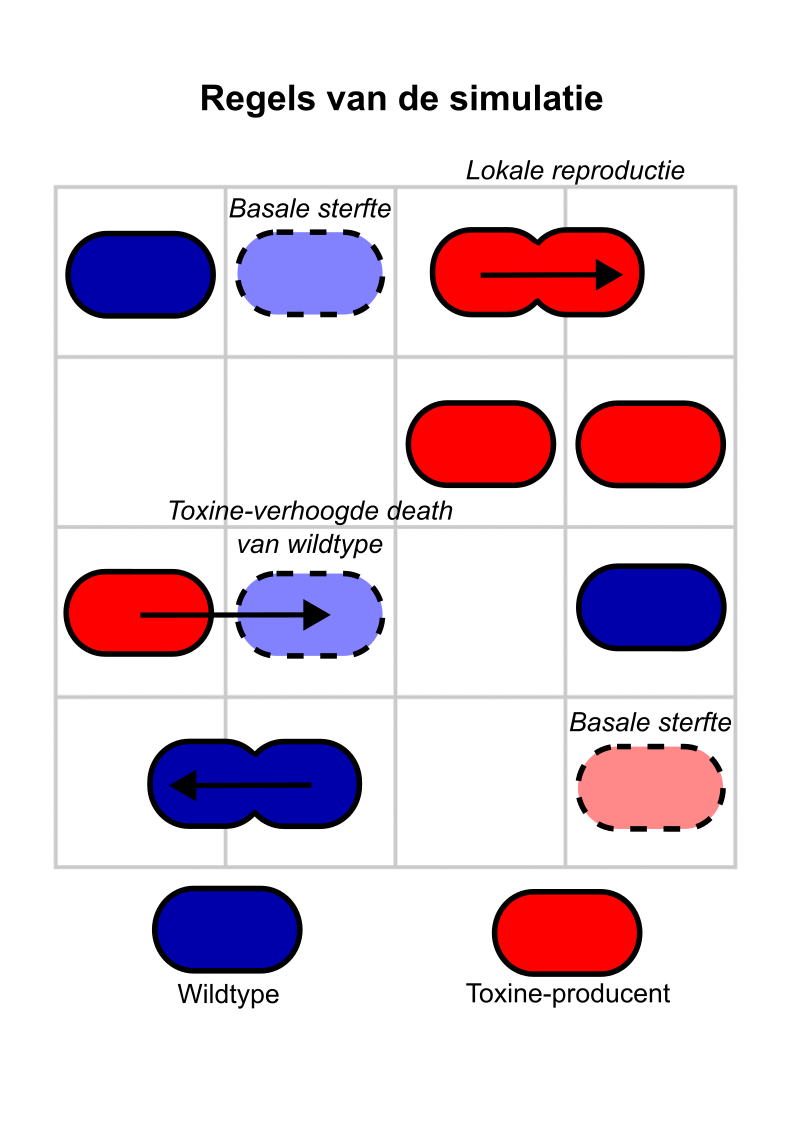
\includegraphics[width=0.6\linewidth,height=\textheight,keepaspectratio]{figuren/project_toxins.png}

Je vindt de simulatie hier:
\url{https://tbb.bio.uu.nl/bvd/bms/simulations/toxins/}.

\begin{enumerate}
\def\labelenumi{\alph{enumi}.}
\setcounter{enumi}{10}
\tightlist
\item
  Bestudeer met de standaard parameters of de toxine-producent kan
  invaderen, en vorm een hypothese over wat er gebeurt.
\item
  Test en bespreek je hypothese met de opties die beschikbaar zijn in de
  simulatie.
\end{enumerate}

\end{tcolorbox}




\end{document}
